\chapter{Математичка позадина}


У претходним поглављима, рад се углавном бавио питањима \textit{шта је ТМ алгоритам и чему  служи}, без улажења у то \textit{\textbf{како}} он уствари ради. 

Опис рада ТМ алгоритама - конкретно LDA имплементације, биће изложен у неколико целина. Најпре ће се објаснити ( увести ) неки  појмови вероватноће који су битни за разумевање сусштине рада алгоритма, а затим ће  бити изнешена математичка позадина самог алгоритма.

\section{Теорија вероватноће}

Теорија вероватноће је математичка дисциплина која се бави изучавањем случајних појава тј. појава чији исходи нису увек строго дефинисани.

Први проблеми који се могу сматрати проблемима вероватноће потичу још из 12. века и везани су за проучавање исхода разних игара на срећу.  Развој \textit{теорије вероватноће} почиње средином 17. века и везан је за имена Блеза Паскала,Пјера де Ферма и Кристијана Хајгенса. Наиме, између Паскала и Ферма је 1654. године започела интересантна преписка о низи проблема међу којима је био и проблем везан за поделу улога приликом прекида једне коцкарске игре. Проблем је био постављен на следеђи начин : Два играча А и Б се договоре да читав улог припадне ономе ко први добије три игре. Када је играч А добио 2 игре а играч Б једну игру, играчи су споразумно одлучили да прекину игру. Поставља се питање како сада да поделе улог. Паскал је предложио поделу у односу 3:1 у корист играча А.
Овај пример често се узима као почетак настанка теорије вероватноће.

Неке од појава које се догађају у реалном свету лако се могу предвидети и објаснити услод познавања законитости њиховог настанка. У такве појаве спадају нпр. помарачење Сунца и Месеца, плима и осека, гравитација итд.
Међутим, постоје појаве чије узроке тренутно није могуће одредити па се не могу у потпуности објаснити и одредити. Неке од таквих појава су нпр. добитак на лутрији или метереолошке појаве.
Прилоком бацања металног, хомогеног новчића, никада није сигрно да ли ће пасти писмо или глава. Међутим, уколико бацамамо новчић много пута, може се уочити да је отприлике исти број пута пало писмо као и глава ( такве експерименте су радили Буфон и Пирсон% - референце! ).
Дакле, законитост код оваквих догађаја може се уочити тек након великог броја понаваљања појаве.

\subsection{Основни појмови}


Основни полазни појам у теорији вероватноће је непразан скуп $\Omega$ који представља скуп свих могућих исхода једног експеримента. Овај скуп се често назива \textbf{простор елементарних догађаја} и може бити коначан, пребројив или непребројив. 
\textbf{Случајни догађаја} или само \textbf{догађај} представља било који подскуп скупа $\Omega$. Најчешће се случајни догађаји означавају великим, штампаним, латиничним словима. За догађај \textbf{А} каже се да се \textbf{реализовао} ако се реализовао неки исход $\omega$ који припада скупу А. Догађај који је садржи све могуће елементарне исходе експеримента назива се \textbf{сигуран догађај} а догађај који не садржи ни један елементарни исход назова се \textbf{немогућ догађај}.


\textit{Пример:}
Нека је дата хомогена коцка чије су стране означене бројевима од 1 до 6. Елементарни догађаји су појављивање одређеног броја при бацању коцкице. Према томе, скуп свих могућих исхода екперимента бацања коцкице је $ \Omega = \lbrace 1,2,3,4,5,6 \rbrace $. Догађај A = "пао је паран број" одређује скуп $ $А$ = \lbrace 2,4,6 \rbrace $


\textbf{Производ два догађаја} $ А $ и $ В $, у ознаци $ AB $ је догађај који се реализује ако и само се ако реализују оба догађаја. Дакле, производ догађаја је пресек скупова А и В. Уколико су А и В дисјунктни скупови (пресек је празан скуп) за такве догађаје кажемо да су \textbf{несагласни} или да се \textbf{искључују}.

\textbf{Збир два додгађаја} А и В, у ознаци $ A \cup B $ представља догађај који се реализује ако се реализује бар један од догађаја А и В. 

\textbf{Разликом догађаја} А и В, у ознаци $ A -  B $ назива се догађај који се реализује ако и само ако се реализује догађај А  а не реализује догађај В. 

\textbf{Потпун систем догађаја} : За догађаје $ A_1,A_2,..A_n$ се каже да образују \textit{потпун систем догађаја} уколико важи : $ \bigcup_{i} A_i = \Omega $ . Дакле, при реализацији неког експеримента бар један од догађаја $ A_1,A_2,..A_n$ ће се реализовати. Посебно су интересантни потпуни системи несагласних догађаја као што се може видети код формуле тоталне вероватноће.

\begin{de}
[Класична дефиниција вероватноће] : Нека је $ \Omega = \lbrace \omega_1,\omega_2,...,\omega_n \rbrace $ скуп свих могућих једнаковероватних елементарних догађа који су међусобно несагласни и нека је $ A = \lbrace \omega_{i_1}, \omega_{i_2}, ... , \omega_{i_m} \rbrace $ догађај који се састоји од \textit{m} елементарних једнаковероватних догађаја. Вероватноћа наступања догађаја А је :
\begin{equation}
 P(A) = \frac{m}{n} 
\end{equation}
\end{de}

 Претходна дефиниција може се неформално изразити и овако : вероватноћа догађаја A једнака је количнику броја \textbf{повољних исхода} експеримена ( исходи када се реализује догађај А ) и укупног броја свих могућих исхода експеримента.

Класична дефиниција вероватноће је применљива само онде где су елементарни догађаји једнаковероватни. Међутим, тај услов је у пракси јако тешко испунити. Чак и у случајевима када је то наизглед очигледно, као што је бацање коцкице, једнаковероватност не може бити гарантована.  Разлози за то могу бити технологија израде коцкице која не мора бити савршено прецизна, немогућност обезбеђивања идеалних и непромењљивих услова током извођења експеримента итд. Због тога је једини начин којим је могуће заиста утврдити вероватноћу догађаја А \textit{статистички приступ} заснован на великом броју експеримената.




\begin{de}
[Статистичка дефиниција вероватноће] : 
Нека се  у $n$ понављања експеримента изведених под приближно истим условима догађај А реализовао ${m_n}$ пута. Вероватноћа догађаја А је
\begin{equation}
 P(A) = \lim_{n\to\infty}\frac{m_n}{n} 
\end{equation}
\end{de}

\subsection{Условна вероватноћа}

Вероватноћа догађаја чија реализација \textbf{не зависи} од наступања било ког другог догађаја назива се \textbf{безусловна вероватноћа}. Ако је реализација догађаја А условљена реализацијом неког догађаја В при чему В није немогућ догађај ( $ P(B) \neq 0 $), тада се вероватноћа догађаја под условом да се десио догађај В назива \textbf{условном вероватноћом} и означава се са 
$ P(A \mid B )$. Дакле, $ P(A \mid B )$ је вероватноћа догађаја А под условима који сигурно доводе до реализације догађаја В.

Нека се изводи експеримент у коме постоји $n$ једнаковероватних елементарних догађаја и нека је са $n_A,n_B,n_{AB}$ означен број елеменгтарних догађаја који доводе до реализације догађаја $A, B ,AB$ редом. 

Према класничној дефиницији вероватноће, вероватноћа реализације догађаја А и АВ је :
\begin{equation}
P(B) = \frac{n_B}{n}, P(AB) = \frac{n_{AB}}{n}
\end{equation}
Ако је реализација догађаја А условљена реализацијом догађаја В, то је број повољних исхода догађаја А $n_{AB}$ (број елементарних догађаја који имају осбине и скупа А и скупа В ). Пошто се догађај А реализује само ако се реализовао догађај В, број свих могућих исхода је $n_B$ (број свих могућих елементарних догађаја када наступа догађај В). Дакле, условна вероватноћа догађаја А, под условом да се десио догађај В је :

\begin{equation}
 P( A \mid B ) = \frac{n_{AB}}{n_B} = \frac{\frac{n_{AB}}{n}}{\frac{n_B}{n}} = \frac{P(AB)}{P(B)} \quad ,  P(B) \neq 0
\end{equation}

У случају да је догађај В условљен догађајом А, аналогно се изводи да је 

\begin{equation}
 P( B \mid A ) = \frac{P(AB)}{P(A)} \quad ,  P(A) \neq 0
\end{equation}

Из релација (3.4) и (3.5) следи

\begin{equation}
 P( AB ) = P(B)\cdot  P( A \mid B ) = P(A)\cdot  P( B \mid A ) 
\end{equation}

Релација (3.6) назива се још и \textbf{теорема о производу вероватноћа}

\begin{te}
[Формула тоталне вероватноће] : 
Ако су $H_1,H_2,..,H_n$ међусобно несагласни догађаји, $P(H_i) > 0 (i=1,..,n)$ при чему важи $H_1+H_2+..+H_n = \Omega $ тада је :
\begin{equation}
	 P(A) = \sum_{i=1}^n P(H_i)P(A \mid H_i)  \textrm{ за сваки догађај}  A \subseteq  \Omega 
\end{equation}
\end{te}
Напомена : Догађаји $H_1,H_2,..,H_n$ чине потпун систем несагласних догађаја.

\begin{dok}
Обзором да су догађаји подскупови скупа свих елементарних догађаја очигледно је да важи

\begin{equation}
A = A\Omega = A \sum_{i=1}^n H_i = \sum_{i=1}^n AH_i. 
\end{equation}
На основу релације (3.6) следи :

\begin{equation}
P(A) = P(\sum_{i=1}^n AH_i) = \sum_{i=1}^n P(AH_i) = \sum_{i=1}^n P(H_i)P(A \mid H_i)
\end{equation}
\end{dok}

Вероватноће $P(H_i)$ су обично познате унапред и називају се \textbf{априорним вероватноћама} а сами догађаји \textbf{хипотезама}. 

\begin{te}
[Бајесова формула \footnote{енг. Bayes} ] : 
Ако су $H_1,H_2,..,H_n$ међусобно несагласни догађаји, $P(H_i) > 0        (i=1,..,n)$ при чему важи $H_1+H_2+..+H_n = \Omega $ тада је :
\begin{equation}
	 P(H_i \mid A ) = \frac{P(H_i)P(A \mid H_i)}{ \sum_{j=1}^n P(H_j)P(A \mid H_j)}  \quad   (i=1...n)  \quad  \textrm{ за сваки догађај}  A \subseteq  \Omega 
\end{equation}
\end{te}

\begin{dok}
Из релације (3.6) следи :

\begin{equation}
P(H_iA) = P(H_i)P(A \mid H_i) = P(A)P(H_i \mid A) \quad  (i=1...n)
\end{equation}
Условна вероватноћа догађаја $H_i$ под условом да се десио догађај А је:
$$ P(H_i \mid A) = \frac{P(H_iA)}{P(A)} = \frac{P(H_i)P(A \mid H_i) }{P(A)} $$

Примењујући формулу потпуне вероватноће за $P(A)$  добија се 
$$
 P(H_i \mid A ) = \frac{P(H_i)P(A \mid H_i)}{ \sum_{j=1}^n P(H_j)P(A \mid H_j)}
$$
што представља Бајесову формулу.

\end{dok}

\subsection{Случајне променљиве}

Ако се сваком елементарном догађају придружи један реалан број, онда се извођење експеримента може посматрати као избор вредности једне променљиве. Променљива величина која 
 те бројене вредности узима са одређеним вероватноћама назива се \textit{случајна променљива}. Дакле, уместо вербалне карактеризације догађаја ( описа речима шта догађај представља ) много је једноставније за рад догађаје окарактерисати бројним вредностима тј. неким реалним бројевима.

\textit{Пример 1 :} У екпериманту бацања новчића могућа су два елементарна исхода : грб или писмо. Нека је догађај који се посматра "пало је писмо". Појава писма се може означити бројем 1 а појава грба бројем 0. Сада се овај екперимент може замислити као избор 0 или 1 са вероватноћом $\frac{1}{2}$

\textit{Пример 2 :} Новчић се баца два пута. Нека је са P означена појава писма а са G појава грба. Скуп свих елементарних исхода екперимента је $ \Omega = \lbrace PP,PG,GP,PP \rbrace$ . Нека је догађај који се посматра "број палих писама". Сваком исходу се може доделити један реалан број и то $ PP -> 2, GP -> 1,PG -> 1, GG ->0$. Ово додељивање вредности се карактерише случајном променљивом.  Случајна променљива сваку од ових вредности узима са различитом вероватнићом.  

\begin{figure}[H]
    \centering
   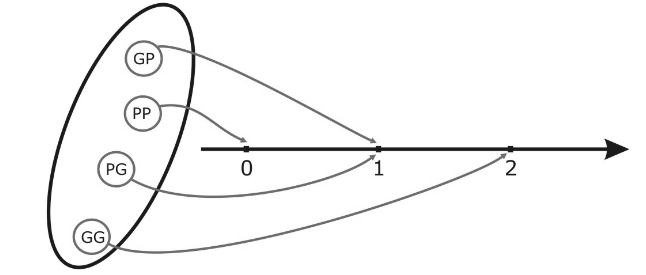
\includegraphics[scale=0.5]{./Slike/slika12.png} 
	\caption{Графички пример случајне променљиве}
	\label{fig:slika12}
\end{figure}

\begin{de}
Функција Х која сваком случајном догађају $\omega \in \Omega $ додељује неки реалан број $X(\omega)$ назива се \textbf{случајна променљива} где је $X:\Omega \longrightarrow R $
\end{de}

Дакле, случајна променљива је пресликавање скупа $\Omega $ у скуп \textbf{реалних} бројева за разлику од вероватноће која је пресликавање скупа  
$\Omega $ у скуп $ [0,1]$

Важно је уочити да случајна променљива \textbf{нема конкретну вредност} већ се само говори о вероватноћама да узме неки конкретну вредност.

Разликују се два основна типа случајних променљивих - \textbf{дискретне} и \textbf{непрекидне}. Подела се врши у зависности од тога да ли случајна променљива узима вредности у пребројивом или непребројивом скупу вредности.



\subsubsection{Дискретне случајне променљиве}

За случајну променљиву се каже да је дискретног типа ако узима коначан број изолованих вредности или пребројиво много вредности

\begin{de}
Нека случајна променљива Х може да узме вредности $x_1,x_2, ... , x_n$ са вероватноћама $p_1,p_2, ... ,p_n$ при чему важи да је $p_1 + p_2 + ... + p_n = 1$. Скуп парова $(x_i,p_i = P\lbrace X=x_i \rbrace), i=1,2,...,n$ или написано :
$$ 
\left(
\begin{array}{ccc}
x_1 & x_2 & \cdots \\
p(x_1) & p(x_2) & \cdots \\
\end{array}
\right)
$$

чине закон расподеле  или распоред вероватноћа случајне променљиве Х.
\end{de}

\textit{Закон расподеле случајне промнљиве} може да се посматра као \textbf{правило} по коме се свакој вредности случајне променљиве придружује одговарајућа вероватноћа. Дакле, при реализацији експеримента сигурно ће се десити догађај којем је придужена нека вредност случајне променљиве. Због тога је сума свих вероватноћа у расподели случајне променљиве 1. Међутим, нису све вредности подједнако вероватне па се свакој вредноти придружује вероватноћа са којом се очекује.
Претходна дефиниција може се интерпретирати и на следећи начин : извесна маса једнака јединици је распоређена на такав начин да се у тачкама $x_1,x_2, ... , x_n$ налазе одговарајући делови масе $p_1,p_2, ... ,p_n$. Услед оваквог тумачења, закон расподеле вероватноћа се често назива и \textbf{функција масе вероватноћа}

У примеру 2, случајна променљива може да узме три вредности, тј. писмо се може појавити 0,1 или 2 пута у два бацања. Ни један други исход није могућ - нпр. у два бацања писмо не може да се појави 3 пута или -1 пут. Међутим, вероватноћа да се писмо неће појавити ни једном (или да се појави два пута) је $\frac{1}{4}$ - вероватноћа да падне глава у првом бацању је $\frac{1}{2}$ и вероватноћа да падне глава у другом бацању је   $\frac{1}{2}$, дакле, вероватноћа да оба пута падне глава је је  $\frac{1}{2} \cdot \frac{1}{2} = \frac{1}{4}$, вероватноћа да се писмо појави тачно једном је $\frac{1}{2}$ - писмо пада тачно једном у случају PG или GP. Вероватноћа за оба ова догађаја је $\frac{1}{4}$. Дакле, вероватноћа да се десио бар један од ових догађаја је  $\frac{1}{4} + \frac{1}{4} = \frac{1}{2}$. Према томе, расподела случајне променљиве "број појављивања писма у два бацања " је :


$$ 
\left(
\begin{array}{ccc}
0 & 1 & 2 \\
\frac{1}{4} & \frac{1}{2} & \frac{1}{4} \\
\end{array}
\right)
$$

Закон расподеле дискретне случајне променљиве може се представити графички, као на следећој слици :

\begin{figure}[H]
    \centering
   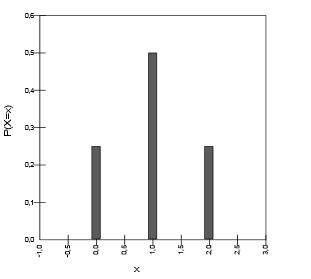
\includegraphics[scale=0.8]{./Slike/slika13.png} 
	\caption{Графички пример случајне променљиве}
	\label{fig:slika13}
\end{figure}

На апсциси се налазе могуће вредности случајних променљивих док се на ординати налазе вероватноће са којом случајна променљива узима дату вредности. Са претходне слике јасно се уочава дискретност посматране случајне променљиве - вероватноћа да случајна промељива узме вредност између неке две целобројне вредности је 0. 
\\
\\

\textbf{Функција расподеле дискретне случајне 
променљиве:}
\\

Распоред или закон расподеле случајне променљиве дискретног типа може се представити као листа свих могућих вредности случајне променљиве и одговарајућих вероватноћа. Међутим, поставља се питање како представти случајну променљиву која може узимати јако пуно вредности тј. бесконачно много вредности. У овом случају би требало формирати листу од бесконачно много чланова, што је практино неизводљиво. (Пример једне такве случајне променљиве би био - број бацања коцкице док се не добију две узастопне шестице. Случајна променљива може узети вредности 2,3,4,... са различитим вероватноћама, при чему не постоји горња граница броја бацања при којој се сигурно добијају две узастопне шестице ).
Због описаног проблема, потребно је пронаћи другачији начин представљања случајне променљиве и одговарајућих вероватноћа. То се постиже \textbf{функцијом расподеле} која се може дефинисати за сваку случајну променљиву.

\begin{de}
\textbf{Функција расподеле} ( још се назива и \textbf{кумулативна функција расподеле}) дискретне случајне променљиве претставља вероватноћу да случајна променљива Х узме вредност која је мања или једнака неком реалном броју $x$ при чему је дефинисана за свако реално   $x$. 
$$ F(x) = P (X<x) \quad \forall x \in R $$
\end{de}

Дакле, кумулативна функција расподеле има облик

$$
F(x) = \left\lbrace
\begin{array}{rl}
0, & x \leq x_1 \\
p_1, & x_1 < x \leq x_2 \\
p_1 + p_2, & x_2 < x \leq x_3 \\
.... & ... \\
1 & x > x_n
\end{array}
\right.
$$

и може се изразити као :

$$
F(x) = \sum_{k,x_k<x} P(X = x_k)
$$

а графички приказ је дат на следећој слици :


\begin{figure}[H]
    \centering
\captionsetup{justification=centering}
   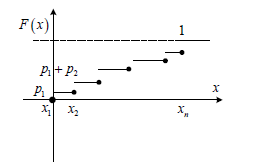
\includegraphics[scale=0.8]{./Slike/slika14.png} 
	\caption{График кумулативне функције расподеле \\ случајне променљиве дискретног типа} 
	\label{fig:slika13}
\end{figure}

Две најважније дискретне расподеле су \textbf{Биномна} и \textbf{Пуасонова} расподела.

\subsubsection{Непрекидне случајне променљиве}
Случајна променљива је (апсолутно) непрекидног типа ако може да узме \textbf{било коју } вредност из неког интервала. Број вредности које може да узме случајна променљива непрекидног типа је \textbf{бесконачан}. Неки од примера су : висина и тежина људи, дужина трајања батерије итд.
На пример, нека је Х случајна променљива која представља дужину рада сијалице. Ова случајна променљива може узети било коју вредност на интервалу од 1 до нпр. 1000 сати. Како у интервалу $[0,1000]$ има бесконачно много реалних бројева, не постоји начин да се дефинише вероватноћа за сваку појединачну вредност, као што је био случај код дискретних променљивих. Такође, интуитивно је јасно да је вероватноћа да ће сијалица прегорети у тачно одређеном тренутку једнака 0  док је вероватноћа да ће прегорети у неком временском интервалу различита од нуле.


\begin{de}
Случајна променљива X је апсолутно непрекидног типа ако постоји \textbf{ненегативна} функција $ f: \mathbb{R} -> \mathbb{R}$ таква да за било који интервал $[a,b] \subset (- \infty,\infty)$ важи :
\begin{equation}
P \lbrace a \leq X < b \rbrace = \int\limits_{a}^{b} f(x)dx
\end{equation}
\end{de}

Функција $f(x)$ мора да задовољи услов : 
$$
P \lbrace - \infty \leq X <  \infty \rbrace = P \lbrace \Omega \rbrace =  \int\limits_{- \infty}^{\infty} f(x)dx  = 1
$$

Функција $f(x)$ се назива \textbf{густина расподеле вероватноће} случајне променљиве Х.
Случјане променљиве \textbf{дискретног типа } немају густину расподеле баш као што ни случајне променљиве непрекидног типа немају закон расподеле вероватноћа.

Из релације (3.12) следи да је вероватноћа да случајна променљива узме вредност из интервала  $[a,b]$ једнака \textbf{површини} испод графика функције $f(x)$ на интервалу $[a,b]$.




\begin{figure}[H]
    \centering
\captionsetup{justification=centering}
   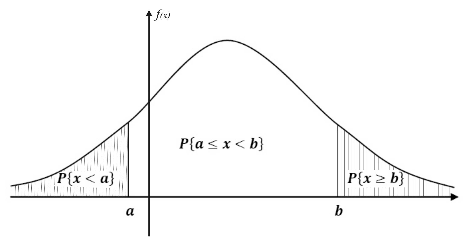
\includegraphics[scale=0.8]{./Slike/slika15.png} 
	\caption{Функција густине} 
	\label{fig:slika13}
\end{figure}


\textbf{Функција расподеле непрекидне случајне 
променљиве:}



\begin{de}
\textbf{Функција расподеле} (\textbf{кумулативна функција расподеле}) непрекидне случајне променљиве се може представити као :

$$
F(x) = P (X \leq x) = \int \limits_{-\infty}^{x} f(t)dt) \quad x \in (-\infty,\infty) 
$$
где је $f(x)$ функција густине.
\end{de}

Дефиниција кумулативне суме  преко интеграла је јаснија ако се има на уму интервал из ког случајна променљива може да узме вредности. Код случајних променљивих дискретног типа, тај скуп је био пребројив па се кумулативна функција расподеле дефинисала преко суме. Случајне променљиве непрекидног типа могу узти бесконачно много вредности па се сума код дискретних случајних променљивих ( када број тачака тежи у бесконачност) замењује интегралом.

Напомена : Ако случајна променљива Х не узима све вредности из интервала $ (-\infty,\infty) $ усваја се да је $f(x) = 0$ за све вредносто $x$ из интервала у којима Х не узима вредности.

График кумулативне функције расподеле непрекидне случајне променљиве Х је сада представљен глатком кривом линијом ( за разлику од случајне променљиве дискретног типа где је график био "степенаст" ).


\begin{figure}[H]
    \centering
\captionsetup{justification=centering}
   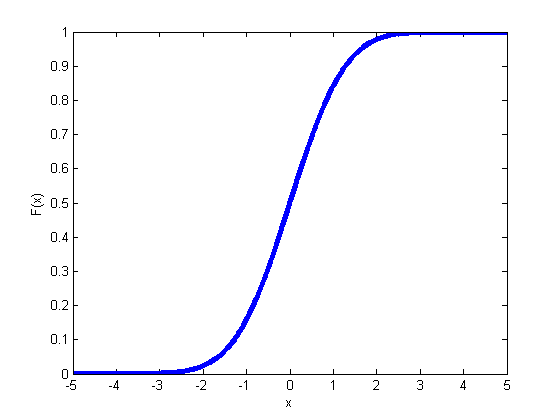
\includegraphics[scale=0.5]{./Slike/cdf.png} 
	\caption{Кумулативна функција расподеле \\ за случајне променљиве непрекидног типа} 
	\label{fig:slika13}
\end{figure}



\subsubsection{Вишедимензионалне случајне прменљиве}

Случајна променљива представља пресликавање скупа догађаја у реалне бројеве. Дакле, излази експеримента се мапирају у једнодимензионалан простор реалних бројева. Међутим, постоје случајеви када је потребно излазе експеримента мапирати у вишедимензионалне реалне просторе. На пример, при истовременом бацању два новчића могућа су 4 исхода :
\begin{enumerate}
\item $s_1$: први новчић писмо - други новчић писмо
\item $s_2$: први новчић писмо - други новчић глава
\item $s_3$: први новчић глава - други новчић писмо
\item $s_4$: први новчић глава - други новчић глава
\end{enumerate}

Нека је са $X_1$ означена случајна променљива која узима вредност 1 ако се на првом новчићу појавила глава, односно 0 ако се појавило писмо и аналогно $X_2$ која на исти начин означава појаву главе на другом новчићу. Исход експеримента се сада може описати дводимензионалном променљивом $(X_1,X_2)$. Графички приказ ове дводимензионалне промељиве дат је на следећој слици :

\begin{figure}[H]
    \centering
\captionsetup{justification=centering}
   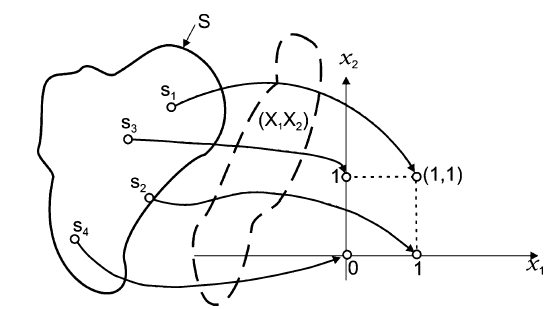
\includegraphics[scale=0.8]{./Slike/slika17.png} 
	\caption{Експеримент :  бацање два новчића. \\ Скуп $S$ представља скуп свих елементарних исхода ( $\Omega$)} 
	\label{fig:slika17}
\end{figure}





\begin{de}
Ако су $X : \Omega -> \mathbb{R} , Y : \Omega -> \mathbb{R}$ случајне променљиве, тада се \textbf{уређени пар} $(X,Y)$ натива \textbf{дводимензионална случајна променљива}. Уређеним паром   $(X,Y)$ се  сваком исходу  $\omega \in \Omega$ придружује уређени пар бројева $(X(\omega),Y(\omega))= (x,y) \in \mathbb{R} \times \mathbb{R} = \mathbb{R}^2$.
\end{de}

На следећој слици графички је представљена дводимензионална случајна применљива.



\begin{figure}[H]
    \centering
\captionsetup{justification=centering}
   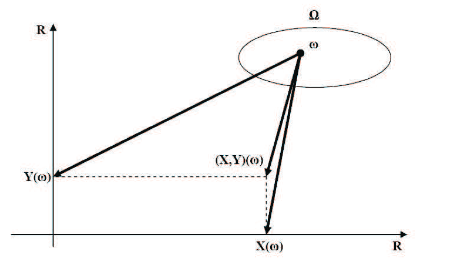
\includegraphics[scale=0.8]{./Slike/slika16.png} 
	\caption{Дводимензионална случајна променљива} 
	\label{fig:slika13}
\end{figure}

Овако уведен појам дводимензионалне случајне променљиве се може проширити и на више димензија и тада настају $n$-димензионалне случајне променљиве. Закључци изведени за дводимензионалне се такође односе и на вишедимензионалне случајне приоменљиве.

\textbf{Кумулативна функција расподеле} ( још се назива и \textit{заједничка расподела енг. joint distribution} дводимензионалне случајне променљиве, у ознаци $ F_{XY} : \mathbb{R}^2 -> [0,1] $ дефинише се као вероватноћа реализације догађаја $ \lbrace X \leq x , Y \leq y \rbrace $ односно :
$$
F_{X,Y}(x,y) = P \lbrace X \leq x, Y \leq y \rbrace \quad  - \infty < x,y < \infty
$$

Неке карактеристике функције расподеле дводимензионалне случајне променљиве :

\begin{enumerate}

\item  $ 0 \leq F_{X_1,X_2}(x_1,x_2) \leq 1 $
\item  $ F_{X_1,X_2}(-\infty,-\infty) =0 $
\item  $ F_{X_1,X_2}(-\infty,-\infty) =0 $  \\
$ F_{X_1,X_2}(-\infty,x_2) =0 $
$ F_{X_1,X_2}(x_1,-\infty) =0 $
\item  $ F_{X_1,X_2}(\infty,\infty) =1 $
\item  \begin{equation}
F_{X_1,X_2}(x_1,\infty) = F_{X_1}(x_1) 
\end{equation} 
\item 
\begin{equation}
F_{X_1,X_2}(\infty,x_2) = F_{X_2}(x_2) 
\end{equation} 

\end{enumerate}


Једнакостима (3.13) и (3.14) су дефинисане \textbf{маргиналне расподеле} случајних променљивих $X_1$ и $X_2$. Маргиналне расподеле су уствари расподеле једнодиментионалних случајних променљивих $X_1$ и $X_2$. На следећој слици је предсављена заједничка расподела две случајне приоменљиве заједно са њиховим маргиналним расподелама.

\begin{figure}[H]
    \centering
\captionsetup{justification=centering}
   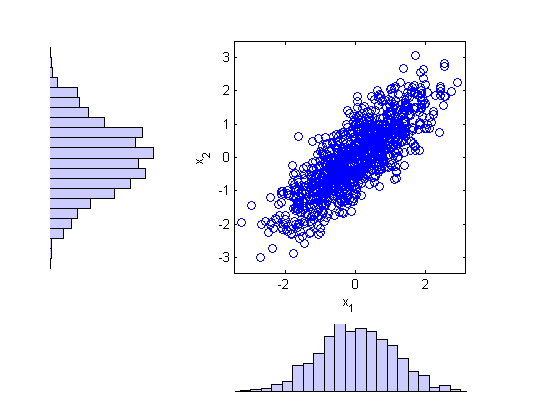
\includegraphics[scale=0.8]{./Slike/slika19.png} 
	\caption{Дводимензионална случајна променљива и маргиналне расподеле} 
	\label{fig:slika13}
\end{figure}


\textbf{Заједничка функција густине} (енг. joint density function) дводимензионалне случајне променљиве се дефинише као :

\begin{equation}
f_{X_1,X_2}(x_1,x_2) = \frac{d^2 F_{X_1,X_2}(x_1,x_2)}{dx_1dx_2}
\end{equation}

У случају једнодимензионалне случајне променљиве, површина испод графика функције густине на неком интервалу предстваљала је вероватноћу да случајна променљива узме вредност из тог интервала. У случају дводимензионалне случајне промељиве од интереса је пронаћи вероватноћу да она узме вредност из неке \textbf{области}. Та вероватноћа представља \textbf{запремину} тела ограниченог функцијом густине са горње стране и датом облашћу са доње стране.

\begin{figure}[H]
    \centering
\captionsetup{justification=centering}
   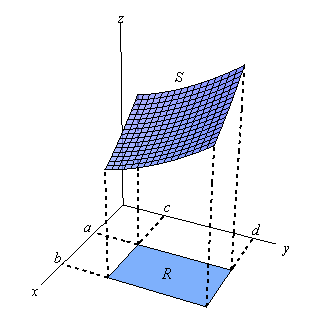
\includegraphics[scale=0.8]{./Slike/slika18.png} 
	\caption{Вероватноћа да дводемнзионална случајна промељива $(X,Y)$ узме вредности из области $R$} 
	\label{fig:slika18}
\end{figure}

 
Неке особине функције густине :

\begin{enumerate}
\item  $ \int \limits_{-\infty}^{\infty}\int \limits_{-\infty}^{\infty} f_{X_1,X_2}(x_1,x_2)dx_1dx_2 = 1$
\item  $F_{X_1,X_2}(x_1,x_2) =  \int \limits_{-\infty}^{x_1}\int \limits_{-\infty}^{x_2} f_{X_1,X_2}(x_1,x_2)dx_1dx_2$
\item  $F_{X_1}(x_1) =  \int \limits_{-\infty}^{x_1}\int \limits_{-\infty}^{\infty} f_{X_1,X_2}(x_1,x_2)dx_1dx_2$ \\
$F_{X_2}(x_2) =  \int \limits_{-\infty}^{x_2}\int \limits_{-\infty}^{\infty} f_{X_1,X_2}(x_1,x_2)dx_1dx_2$ 
\item $f_{X_1}(x_1) =  \int \limits_{-\infty}^{\infty} f_{X_1,X_2}(x_1,x_2)dx_2$ \\
$f_{X_2}(x_2) =  \int \limits_{-\infty}^{\infty} f_{X_1,X_2}(x_1,x_2)dx_1$ 
\item $P \lbrace x_{11} < X_1 \leq x_{12}, x_{21}<X_2 \leq x_{22} \rbrace =  \int \limits_{x_{21}}^{x_{22}}\int \limits_{x_{11}}^{x_{12}} f_{X_1,X_2}(x_1,x_2)dx_1dx_2 $
	
\end{enumerate}


\textbf{Функција условне расподеле и густине}


У неким специфичним случајевима је потребно пронаћи расподелу једне случајне променљиве знајући вредност друге случајне променљиве. Таква расподела назива се \textbf{условном расподелом} и обележава се са $F_{X_1}(x_1 \mid X_2 = x_2)$ . Аналогно, може се дефинисати и проблем налажења функције густине једне случајне променљиве знајући вредност друге случајне променљиве и таква функција густине  се означава са $f_{X_1}(x_1 \mid X_2 = x_2 )$. Према \cite{verov4} условна расподела односно густина се рачуна по следећем обрасцу ( детаљно извођење се може наћи у \cite{verov4})

$$  F_{X_1}(x_1 \mid X_2 = x_2) = \frac{\int \limits_{-\infty}^{x_1} f_{X_1,X_2}(x_1,x_2)dx_1}{f_{X_2}(x_2)} $$
односно :
$$  f_{X_1}(x_1 \mid X_2 = x_2) = \frac{f_{X_1,X_2}(x_1,x_2)}{f_{X_2}(x_2)} $$




\section{Важније расподеле}
\subsection{Бинонма и полиномна(енг. multivariate ) расподела}

\textbf{Бинонма расподела}

Нека ја А догађај неког екесперимента Е који се реализује са вероватноћом  $P(A) = p$. Тада је вероватноћа супротног догађаја $P(\overline{А}) = 1-p = q$. 
Резултат експеримента који је до интереса је остваривање или неостваривање догађаја А. Дакле, може се сматрати да је скуп свих елементарних исхода $\Omega = \lbrace A, \overline{A} \rbrace$. Нека се експеримент понавља \textbf{независно} и у неизмењеним условима $n$ пута. На тај начин је формиран \textbf{сложени експеримент} чији  скуп елементарних исхода садржи све могуће $n$-торке састављене од $А$ и $\overline{A}$ и има их укупно $2^n$. Нека је, даље, на том скупу елементарних исхода дефинисана случајна променљива $X_n$ као  број остваривања догађаја А у $n$ понављања експеримента Е. Вероватоћа да ова случајна променљива узме конкретну вредност $k$ је :
$$
p_k = P \lbrace X_n = k \rbrace ={ n \choose k} p^kq^{n-k}
$$

Вероватноће $P \lbrace X_n = k \rbrace ,(k=0,1,..,n)$ дефинишу\textbf{ биномну расподелу}, у ознаци $\mathbb{B}(n,p)$ . Ова расподела је дискретног типа а њена функција расподеле(кумулативна) се може изразити као :
$$
F(x)=\left\lbrace
\begin{array}{cc}
0 & , x \leq 0 \\
\sum_{k=0}^{r} {n \choose k} p^kq^{n-k} & 0 < r < n \\
1 & x > n
\end{array}
\right.
$$

Закон расподеле вероватноћа случајне променљиве биномне расподеле приказан је на следећој слици :


\begin{figure}[H]
    \centering
\captionsetup{justification=centering}
   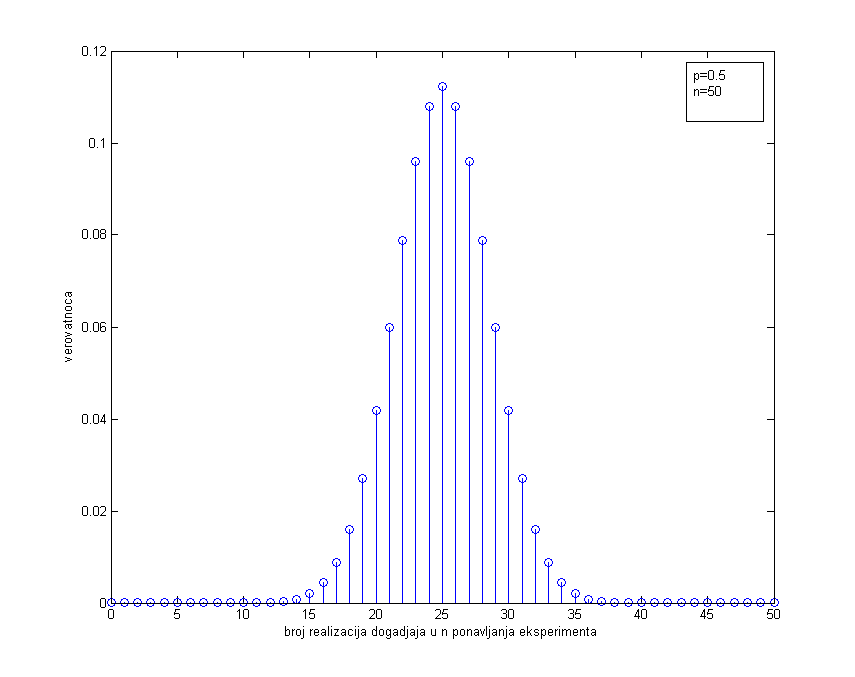
\includegraphics[scale=0.5]{./Slike/slika28.png} 
	\caption{Биномна расподела - закон расподеле} 
	\label{fig:slika20}
\end{figure}

\textbf{Полиномна (енг. multivariate) расподела}

Изводи се серија од $n$ независних експеримената при чему резултат експеримента може бити један од \textbf{коначно много} догађаја : $ A_1,A_2,..,A_k, \sum_{i=1}^k A_i = \Omega, P(A_i)=p_i (i=1,2,..k)$. 
Ако се дефинише $k$-диментионална случајна применљива $(S_n^{(1)},...,S_n^{(k)})$, где $S_n^{(i)}$ предстваља број релаизација случајног догађаја $A_i$ у  $n$ независних експеримената, тада важи :

$$
P(S_n^{(1)}=r_1,..,S_n^{(k)}=r_k) = \frac{n!}{r_1!..r_k!}p_1^{r_1}...p_k^{r_k} $$
$$
r_1,..r_k \in \lbrace 0,1,..,n \rbrace \quad
r_1+..+r_k = n
$$

Ако се са $S = (S_n^{(1)},...,S_n^{(k)})$ означи $k$-диментионална случајна применљива која има полиномијалну расподелу тада се то записује као :
$$
S \sim Mult(n,p)
$$
где је $p = (p_1,p_2,..,p_k)$
Пример полиномне расподеле при чему резулатат експеримента може бити један од \textbf{три} догађаја, дат је на следећој слици :


\begin{figure}[H]
    \centering
\captionsetup{justification=centering}
   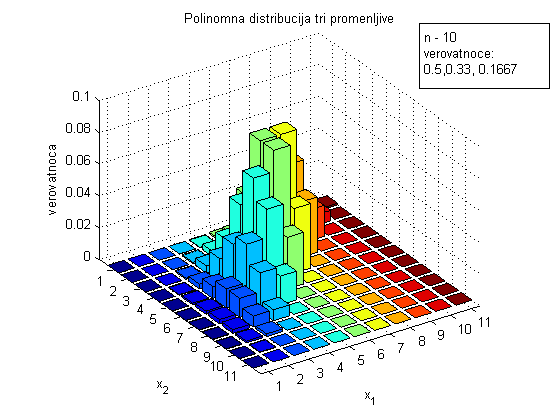
\includegraphics[scale=0.8]{./Slike/slika29.png} 
	\caption{Биномна расподела - закон расподеле} 
	\label{fig:slika20}
\end{figure}


%\subsection{Matrica kovarijanse,disperzija, aritmeticka sredina, multivariate normal distribution, conugate prior}


\subsection{Дирихлеова расподела}

Дирихлеова расподела представља фамилију расподела \textbf{за параметре} $p$  полиномијалне расподеле. Задаје се са :

$$
Dir(p;\alpha) = \frac{1}{B(\alpha)}\prod_{k=1}^{K}p_k^{\alpha_k -1}
$$

при чему је $\alpha$ параметар расподеле а $B$ означава мултиномијалну \textit{бета функцију}. 
Мултиномијалну бета функција се изражава преко гама фунцкије на следећи начин

$$B(\alpha) = \frac{\prod_{i=1}^{|\alpha|}\Gamma(\alpha_i)}{\Gamma(\sum_{i=1}^{|\alpha|}\alpha_i)}$$


На слећој слици је графички предстваљена Дирихлеова расподела за три променљиве :

\begin{itemize}
\item $\alpha = (1,2,3)$
\begin{figure}[H]
\minipage{0.45\textwidth}
  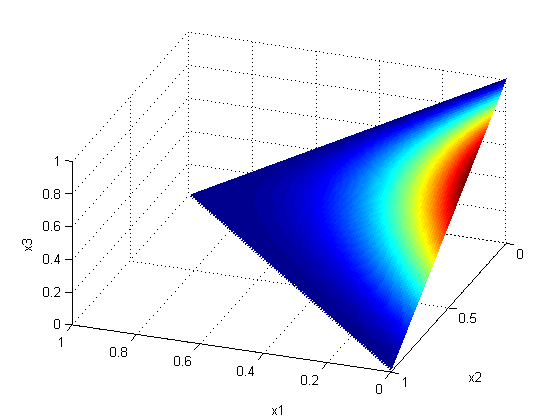
\includegraphics[scale=0.4]{./Slike/slika31.png} 
  \caption{Дирихлеова расподела - интензивнија боја предтсваља већу вероватноћу}\label{fig:slika25}
\endminipage\hfill
\minipage{0.45\textwidth}
  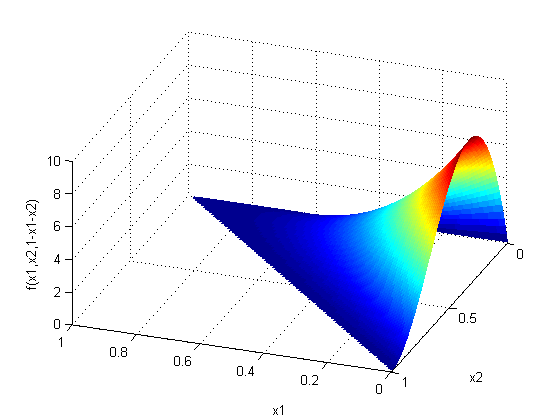
\includegraphics[scale=0.4]{./Slike/slika32.png} 
  \caption{Дирихлеова расподела у три димензије}\label{fig:slika26}
\endminipage\hfill

\end{figure}
\item $\alpha = (1,1,1)$
\begin{figure}[H]
\minipage{0.45\textwidth}
  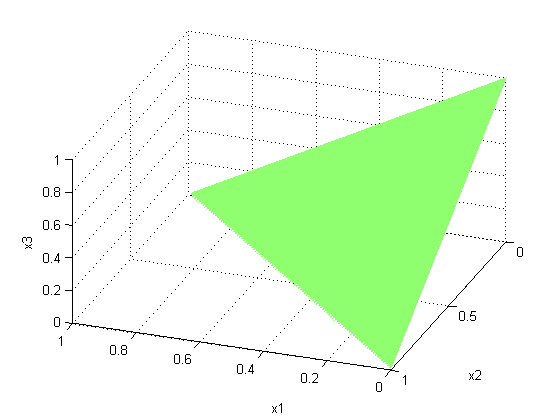
\includegraphics[scale=0.4]{./Slike/slika33.png} 
  \caption{Дирихлеова расподела - интензивнија боја предтсваља већу вероватноћу}\label{fig:slika25}
\endminipage\hfill
\minipage{0.45\textwidth}
  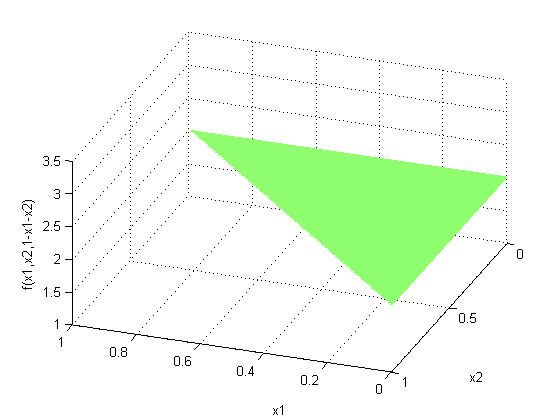
\includegraphics[scale=0.4]{./Slike/slika34.png} 
  \caption{Дирихлеова расподела у три димензије}\label{fig:slika26}
\endminipage\hfill

\end{figure}

\item $\alpha = (3,3,5)$
\begin{figure}[H]
\minipage{0.45\textwidth}
  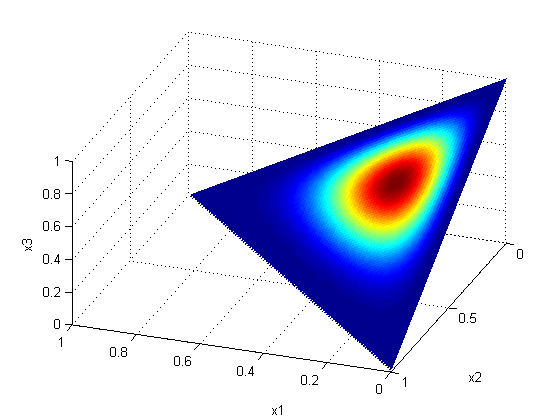
\includegraphics[scale=0.4]{./Slike/slika35.png} 
  \caption{Дирихлеова расподела - интензивнија боја предтсваља већу вероватноћу}\label{fig:slika25}
\endminipage\hfill
\minipage{0.45\textwidth}
  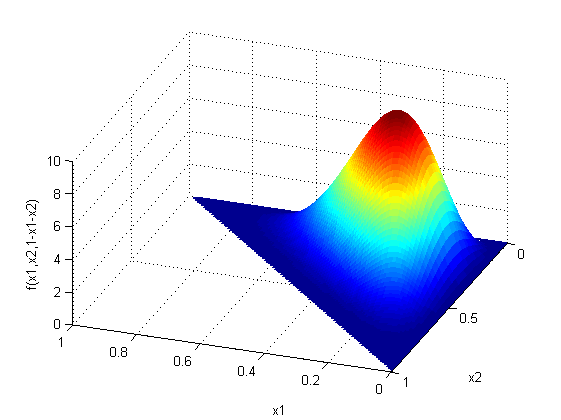
\includegraphics[scale=0.4]{./Slike/slika36.png} 
  \caption{Дирихлеова расподела у три димензије}\label{fig:slika26}
\endminipage\hfill

\end{figure}
\end{itemize}

\section{Гибсово узорковање}
\subsection{Марковљеви ланци}
Марковљевим ланцима моделује се математички сиситем стања и прелаза међу тим стањима. 
\begin{de}
Случајан (стохастички) процес представља математички модел процеса чија је еволуција описана законима вероватноће. \\
Марковљеви процеси су они случајни процеси чије будуће стање зависи само од тренутног стања. Оваква особина још се назива и \textit{одсуство памћења} \\
Марковљеви ланци представљају посебну врсту Марковљевих процеса где се процес може налазити само у коначном броју стања.
\end{de}

Пример Марковљевог ланца дат је на следећој слици :


\begin{figure}[H]
    \centering
\captionsetup{justification=centering}
   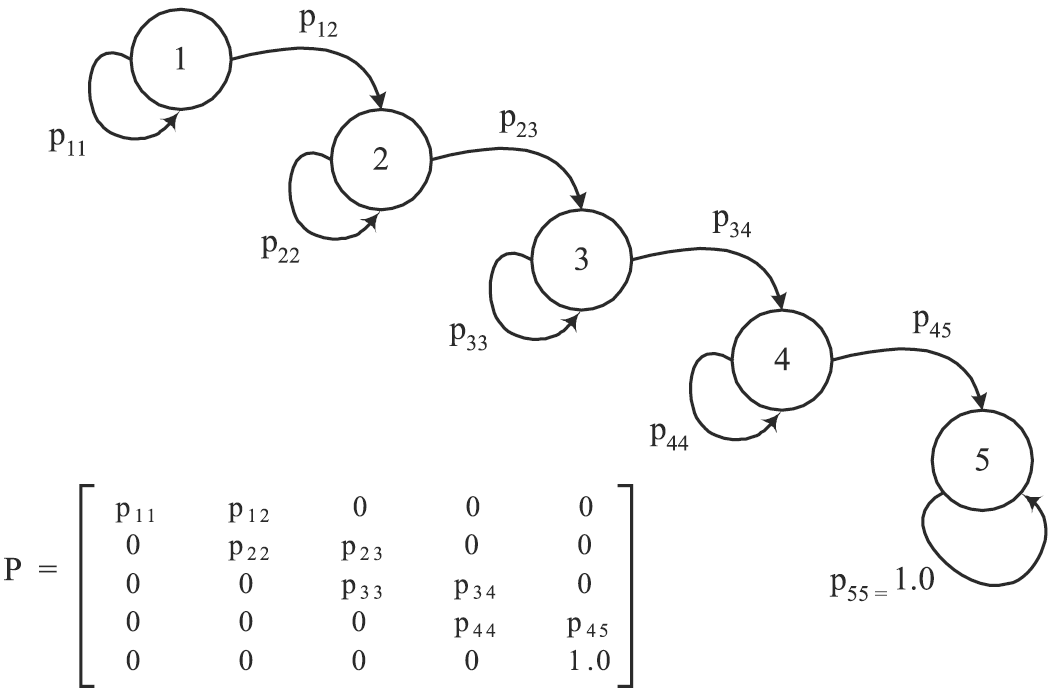
\includegraphics[scale=0.8]{./Slike/slika20.png} 
	\caption{Марковљев ланац - графички пример и матрица транзиције} 
	\label{fig:slika20}
\end{figure}

Систем се састоји од 5 стања. У сваком стању, са одређеним вероватноћама систем може да пређе у неко од следећих стања - конкретно да остане у тренутном стању или да пређе у једно стање ниже. Вероватноћа преласка у следеће стање зависи само од тренутног стања. Марковљеви ланци се често представљају \textbf{матрицама транзиције} при чему $i$-та врста у матрици садржи вероватноће преласка у свако од стање система када се систем налази у стању  $i$. Сума свих вероватноћа у свакој врсти је 1 ( систем сигурно мора да се нађе у неком стању, дакле вероватноћа да систем пређе у неко стање, могуће исто, је 1 ). Свака врста представља условни закон расподеле вероватноћа да систем пређе у било које стање у односу на тренутно стање ( $i$-та врста - $i$-то стање ).
Сака колона представља маргиналну расподелу вероватноћа да се систем нађе у одређеном стању ( $i$-та колона - $i$-то стање ). 


Систем се у једном тренутку може налазити у само једном стању. Нека се стање система карактерише случајном премнљивом  $X_n$ која у тренутку $n$  има расподелу $\overrightarrow{s}$ и нека је укупан број стања система $M$. Расподела $\overrightarrow{s}$ је у ствари закон расподеле (енг. PMF) јер се ради о случајној променљивој дискретног типа - систем може бити само у једном од  $M$ могућих стања, и конкретно може се посматрати као вектор врсте, димензија $1\times M$ где се на $i$ - том месту налази вероватноћа да се систем у тренутку   $n$ нађе у стању $i$.
 
У следећем временском тренутку,  $n+1$, систем се може наћи у било ком од $M$ стања са различитим вероватноћама. Вероватноћа да ће се систем у тренутку  $n+1$  наћи у стању $ј$ означава се са $P(X_{n+1} = j)$. Пошто ова вероватноћа зависи од стања у претходном тренутку, може се изразити на следећи начин ( према формули тоталне вероватноће )
$$
P(X_{n+1} = j) = \sum_{i}^{M} P(X_{n+1}=j \mid X{n}=i)P(X{n}=i) = *  $$
$P(X_{n+1}=j \mid X{n}=i)$ = вероватноћа преласка система из стања i у стање j  -> $p_{i,j} $ \\
$P(X{n}=i)$ = вероватноћа да се систем у тренутку n нађе у стању i -> $s_i$
$$
* = \sum_{i}^{M} p_{i,j}s_{i}
$$
Дакле, верованоћа да систем у  $n+1$-ом тренутку буде у стању $ј$ једнака је суми производа вероватноћа да се систем у $n$ -том тренутку нађе у било ком стању и вероватноћа одговарајућих прелаза. 

Ова сума представља $j$-ту колону у матрици ( димензија $1 \times M$ ) која се добије при множењу вектора  $\overrightarrow{s}$ и матрице транзиције $P$.

Према свему наведеном следи да је закон расподеле случајне променљиве $X_{n+1}$ ( расподела вероватноћа да се систем у  $n+1$-ом тренутку налази у сваком од стања ) једнак $\overrightarrow{s} \times P$.

Аналогно, у тренутку  $n+2$, случајна променљива   $X_{n+2}$ има расподелу  $\overrightarrow{s} \times P^2$, у тренутку $n+3$, случајна променљива   $X_{n+3}$ има расподелу  $\overrightarrow{s} \times P^3$ итд.

\begin{de}
Расподела  $\overrightarrow{s}$ за коју важи : 
$$
\overrightarrow{s} \times P = \overrightarrow{s}
$$
назива се \textbf{стационарна} или \textbf{равнотежна} расподела. 
\end{de}
$\overrightarrow{s} \times P $ представља "један корак у будуђност", тј. расподелу вероватноћа да систем нађе у сваком од стања у следећем временском тренутку. Уколико расподела остаје иста, односно, вероватноће се не мењају са временом, тада се та расподела назива стационарном. Под одређеним условима везаним Марковљеве ланце, доказује се да Марковљев ланац \textbf{увек} конвергира ка својој стационарној расподели без обзира на полазно стање. Више о конвергенцији Марковљевих ланаца може се наћи у \cite{verov6}. Дакле, полазне стање се може изабрати потпуно случајно а затим, уколико се дозвволи да "протекне" довољно времена, закон расподеле вероватноће да се систем нађе у свим стањима система ће конвергирати ка стационарној расподели тог ланца.


\begin{de}
MCMC ( енг. Markov Chain Monte Carlo ) методе представљају класу алгоритама који се користе за синтетичко генерисање узорака случајних променљивих из одговрајућих расподела. Овим методама се креирају Мерковљеви ланаци који као равнотежну расподелу имају расподелу из које се узимају узорци. Једна од MCMC метода је и Гибсово узорковање ( енг. Gibbs sampling )
\end{de}


\textbf{Гибсово узорковање} 

Нека је дата заједничка расподела (енг. joint distribution) $p(\textbf{z})= p(z_1,z_2,..,z_M)$ из које је потрбено одабрати неку вредност (енг. sample ) и нека је познато  почетно стање Марковљевог ланца који је потребно генерисати. Сваки корак Гибсовог узорковања почиње заменом  вредности једне променљиве  $z_1,z_2,..,z_M$ вредношћу која се добија из \textbf{условне расподеле} те променљиве у односу на све остале.  Дакле, $z_i$ се мења вредношћу која се узима из расподеле $p(z_i \mid z_{-i})$, где је са $z_i$ означена $i$-та координата вектора $z$  а са   $z_{-i}$ сви $z_1,z_2,..,z_M$ без $z_i$. Ова процедура се наставља за све променљиве по неком одређеном редоследу. При довољном броју итерација, врсности вектора $z$ ће конвергирати ка $p(z)$.

На пример, нека је дата расподела три случајне променљиве $p(z_1,z_2,z_3)$ и нека су вредности у тренутку $t : z_1^{t},z_2^{t},z_3^{t}$. Нека се замена вредности променљивих врши у односу на индекс, од најмањег ка највећем. Вредност $z_1^{t}$ се мења новом вредношћу  $z_1^{t+1}$ која се узима ( узрокује ) из расподеле 
$$
p(z_1|z_2^{t},z_3^{t}).
$$
Сада се вредност $z_2^{t}$ мења са вредношћу  $z_2^{t+1}$ која се узима из расподеле 

$$
p(z_2|z_1^{t+1},z_3^{t}).
$$

Дакле, одмах се користи нова вредност променљиве $z_1$. Коначно, за промену вредности $z_2^{t}$ користи се вредност $z_3^{t+1}$ која се добија из расподеле :

$$
p(z32|z_1^{t+1},z_2^{t+1}).
$$

Овим је завршена \textbf{једна итерација} Гинбсовог узорковања. Исти процес се наставља кроз низ итерација све до одређеног броја или до неког другог услова заустављања.

Описана процедура се може уопштити и на више од три променљиве и може се представити следећим псеудокодом:

\begin{figure}[H]
    \centering
\captionsetup{justification=centering}
   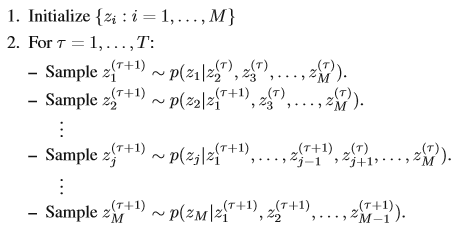
\includegraphics[scale=0.8]{./Slike/slika21.png} 
	\caption{Псеудокод Гибсовог узорковања, преузето са \cite{verov7}} 
	\label{fig:slika20}
\end{figure}


Гибсово узорковање подразумева да су унапред познате  \textbf{условне расподеле} свих променљивих и да је могуће узорковање из њих.

\textit{Пример :} Нека је потребно узорковати вредности из дводимензионалне нормалне расподеле $ \mathcal{N}(\mu, \Sigma )$ Гибсовим узорковањем при чему је 

$$\mu = [\mu_1,\mu_2] = [0,0]$$
$$\Sigma = \left[
\begin{array}{cc}
1 & \rho_{12} \\
\rho_{21} & 1
\end{array}
\right] =  \left[
\begin{array}{cc}
1 & 0.8 \\
0.8 & 1
\end{array}
\right]$$

Графички приказ овакве дводимензионалне нормалне расподеле дат је на следећој слици ( тродимензионално и пројектовано на две димензије ):

\begin{figure}[H]
\minipage{0.45\textwidth}
  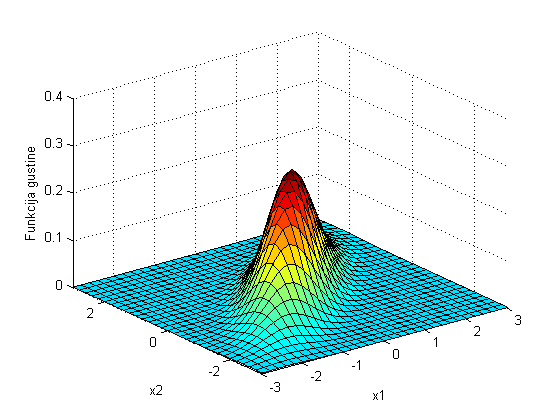
\includegraphics[scale=0.5]{./Slike/slika25.png} 
  \caption{Тродимензионални приказ дводимензионалне нормалне расподеле}\label{fig:slika25}
\endminipage\hfill
\minipage{0.45\textwidth}
  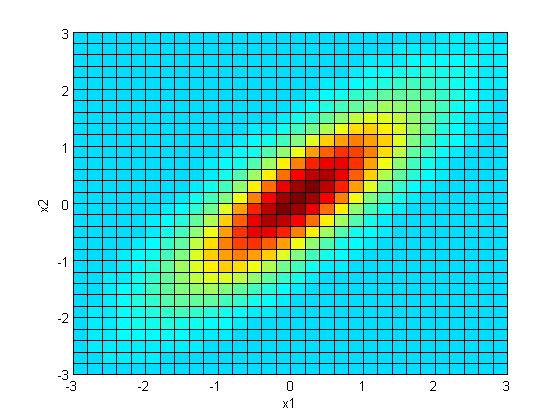
\includegraphics[scale=0.5]{./Slike/slika26.png} 
  \caption{Дводимензионлни приказ дводимензионалне нормалне расподеле}\label{fig:slika26}
\endminipage\hfill

\end{figure}

Основна претпоставка Гибсовог узорковања је да су познате условне расподеле свих променљивих и да је из њих могуће узорковати. Према \cite{verov7} и \cite{verov8}, за условне расподеле дводимензионалне заједничке расподел важи :
$$
p(x_1 \mid x_2^{(t-1)}) = \mathcal{N}(\mu_1 + \rho_{21}(x_2^{(t-1)} - \mu_2),\sqrt{1-\rho_{21}^2})
$$
и
$$
p(x_2 \mid x_2^{(t)}) = \mathcal{N}(\mu_2 + \rho_{12}(x_2^{(t)} - \mu_2),\sqrt{1-\rho_{12}^2})
$$
Дакле, обе условне расподеле представљају једнодимензионалну нормалну расподелу са одговарајућим параметрима.
Почетне вредности променљивих се бирају случајно зато што нису од важности. Марковљев ланац ће свакако конвергирати ка дводимензионалној нормалној расподели са неведеним параметрима после одређеног броја итерација. У зависности од полазног стања, тај број итерација ће бити мањи или већи.

На следећем сликама су предстваљене добијене расподеле Гибсовим узорковањем за различите почетне вредности :


\begin{figure}[H]
\minipage{0.32\textwidth}
  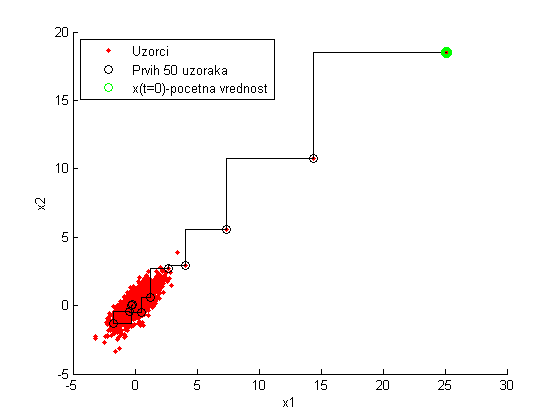
\includegraphics[scale=0.4]{./Slike/slika22.png} 
  \caption{Почетна тачка (25.1284,18.5165)}\label{fig:slika22}
\endminipage\hfill
\minipage{0.32\textwidth}
  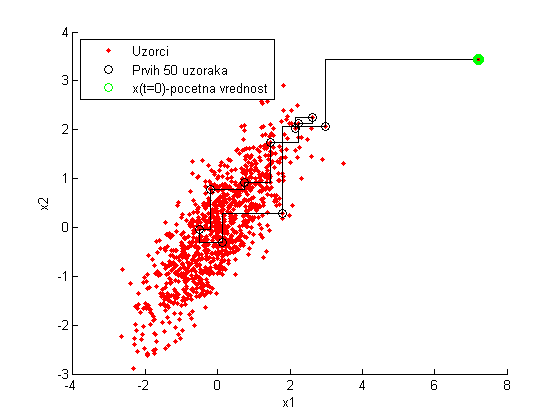
\includegraphics[scale=0.4]{./Slike/slika23.png} 
  \caption{Почетна тачка (7.2162, 3.4380)}\label{fig:slika23}
\endminipage\hfill
\minipage{0.32\textwidth}%
   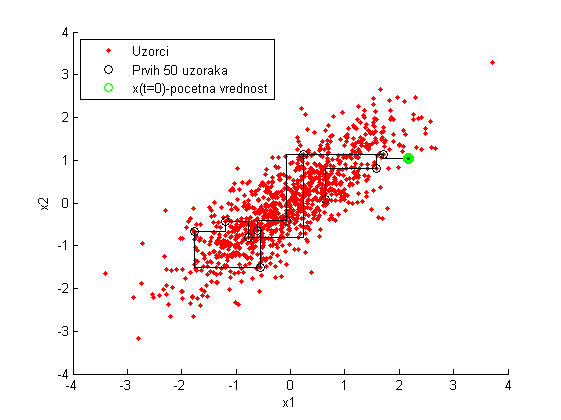
\includegraphics[scale=0.4]{./Slike/slika24.png} 
  \caption{Почетна тачка ( 2.1649, 1.0314)}\label{fig:slika24}
\endminipage
\end{figure}

Са слика је очигледно да се првих неколико узорака може занемарити (\ref{fig:slika22} може се занемарити првих 7-8 узорака).

Важно је приметити да се узимање узорака увек креће по "степенастом" обрасцу. Дакле, две суседне тачке имају исту једну координату ($x$ или $y$). То је зато што  Гибсово узорковање у једном тренутку мења \textbf{само једну} променљиву у односу на одговарајућу вредност друге.

Конвергенција алгоритма Гибсовог узорковања ка стационарној расподели Марковљевог ланца је теоретски загарантована, али је у пракси јако тешко одредити број итерација након којих ланац почиње да конвергира. Један од начина процене конвергенције је и рачунање \textit{log-likelihood} -а

\section{Како ради ТМ алгоритам}

Раније је неформално описан  LDA генеративни процес. Основна претпоставка је да се сваки документ у одређеној пропорцији говори о свакој теми ( има одређену расподелу над темама) као и да свакој теми све речи из корпуса припадају са различитим вероватноћама ( расподела над речима).  Генеративни процес се , према \cite{verov9}, може описати следећим псеудокодом :

\begin{figure}[H]
  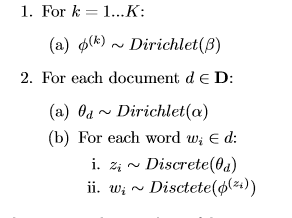
\includegraphics[scale=0.8]{./Slike/slika27.png} 
  \caption{Генеративни процес LDA-а }\label{fig:slika27}
\end{figure}

при чему је :
$K$ - укупан број тема у колекцији
$\phi_{(k)}$ -  расподела над свим речима из колекције и представља расподелу над речима у $k$-тој теми
$\theta_d$ - расподела над темама у документу $d$.
$z_i$ - тема којој припада реч $w_i$.
$\alpha,\beta$ - \textbf{хиперпараметри} тј. параметри симетричних Дирехлеових расподела.

Описани генеративни процес резултује формирањем следеће заједничке расподеле :

\begin{equation}
p(w,z,\theta,\phi \mid \alpha,\beta) = p(\phi \mid \beta)p(\theta \mid \alpha)p(z \mid \theta)p(w \mid \phi_z)
\end{equation}
Непозанте променљиве које је потребно "открити" су $z,\theta$ и $\phi$ на основу (једино) познатих  \textbf{речи} и њиховог присуства у сваком од докумената. Дакле, потребно је пронаћи расподеле наведених променљивих \textbf{под условом} да су познате речи и њихова распоређеност по документима тј. открити њихове постериорне расподеле.
Основни проблем ТМ је  \textbf{постериорно закључивање} (енг. posterior inference) односно отривање постериориних расподела латентних случајних променљивих на основу задатог скупа докумената и речи што представља решавање следеће једначине :

\begin{equation}
p(\theta,\phi,z \mid w,\alpha,\beta) =\frac{p(\theta,\phi,z,w,\mid \alpha,\beta)}{p(w \mid \alpha,\beta)}
\end{equation}

Према  \cite{verov9}, рачунање имениоца овог разломка је готово немогуће па се стога прибегава апроксимативним методама каква је и Гибсово узорковање.

Да би се применило Гибсово узорковање, потребно је познавати  условне расподеле свих променљивих из чије се заједничке расподеле узоркује. Међутим, показује се да је довољно пронаћи само $z$ јер се остале две променљиве могу преко ње израчунати и то (према \cite{verov9}):

$$
\theta_{d,z} = \frac{n(d,z)+\alpha}{\sum_{|Z|}n(d,z)+\alpha}
$$
$$
\phi_{z,w} = \frac{n(z,w)+\beta}{\sum_{|W|}n(z,w)+\beta}
$$
 
Овако примењен алгоритам Гибсовог узорковања назива се још и енг. Collapsed Gibbs Sampling. Дакле, циљ је пронаћи за сваку реч, вероватноћу да припадне свакој од тема, под условом да су познате теме којима припадају остале речи у том тренутку. Формалније, ово се може записати $ p(z_i \mid z_{-i},\alpha,\beta,w)$ где $ z_{-i}$ предстваља доделу тема свим речима сем $i$-те. 

Априорне расподеле коришћене у ТМ су Дирихлеове.Важна особина Дирихлеове расподеле је да је она \textbf{конјугована} са мултиномијалном расподелом. 
Дирихлеова расподела је расподела над параметрима мултиномијалне расподеле. Нека је на почетку претпостављено да параметри мултиномијалне расподеле припадају некој Дирихелеовој расподели - $\mathbf{p} \sim Dir(\mathbf{p,\alpha})$. Нека је $\mathbf{x}$ узорак генерисан из мултиномијалне расподеле $Mult(\mathbf{x;p})$. Тада важи да је постериорна расподела $\mathbf{p}$ ( дакле, расподела под условом да је познат узорак  $\mathbf{x}$ ) такође \textbf{Дирихлеова расподела} са параметром $\mathbf{x+\alpha}$ тј.:
\begin{equation}
p(\mathbf{p\mid x,\alpha}) = Dir(\mathbf{p;x+\alpha}) = \frac{1}{B(\mathbf{x+\alpha}})\prod_{i=1}^{|\mathbf{\alpha}|} p_i^{x_i+\alpha_i-1}
\end{equation}

Како (3.18) представља \textbf{расподелу} то важи да је :

\begin{equation}
1 = \int \frac{1}{B(\mathbf{x+\alpha}})\prod_{i=1}^{|\mathbf{\alpha}|} p_i^{x_i+\alpha_i-1} = \frac{1}{B(\mathbf{x+\alpha}})\int \prod_{i=1}^{|\mathbf{\alpha}|} p_i^{x_i+\alpha_i-1}
\end{equation}
Одакле следи да је :

\begin{equation}
\int \prod_{i=1}^{|\mathbf{\alpha}|} p_i^{x_i+\alpha_i-1} = B(\mathbf{x+\alpha})
\end{equation}

Ова једнакост је важна за даљи опис рада ТМ алгоритма.

Према формули условне расподеле, важи :


\begin{equation}
p(z_i \mid z_{-i},\alpha,\beta,w) = \frac{p(z_i,z_{-i},w \mid \alpha,\beta)}{z_{-i},w \mid \alpha,\beta)} \propto p(z_i,z_{-i},w \mid \alpha,\beta) = p(z,w \mid \alpha,\beta)
\end{equation}

$p(z,w \mid \alpha,\beta)$ се може посматрати као "маргиналан расподела" две променљиве  заједничке расподеле (3.16)  па важи :

\begin{equation}
p(z,w \mid \alpha,\beta) = \iint p(z,w,\theta,\phi \mid \alpha,\beta)d\theta d\phi = \iint p(\phi \mid \beta)p(\theta \mid \alpha)p(z \mid \theta)p(w \mid \phi_z) d\theta d\phi 
\end{equation}

Груписањем по заједночкој зависној променљивој, претхонда једначина се може написати :

\begin{equation}
p(z,w \mid \alpha,\beta) = \int p(z \mid \theta)p(\theta \mid \alpha)d\theta \int p(w \mid \phi_z)p(\phi \mid \beta)d\phi
\end{equation}

Оба интерграла представљају комбинацију узорка из мултиномијалне расподеле и априорне Дирихлеове расподеле. Како је Дирихлеова расподела конјугована (conjugate prior) са мултиномијалном, у подинтегралном изразу се налази "множење" две Дирихлеове расподеле са одговарјућим параметрима.

Дакле :
Пошто  $p(z \mid \theta)$ има мултиномијалну дистрибуцију, важи:
\begin{equation}
p(z \mid \theta) = \prod_{i=1}^D \prod_{k=1}^K \theta_{d,k}^{\Omega_{d,k}}
\end{equation}
, где је $\Omega_{d,k}$ број који означава колико пута је тема $k$ додељена у документу $d$ - број речи који у документу $d$ припадају теми $k$.

Члан $p(\theta \mid \alpha)$ је из основне Дирихлеове расподеле па важи :

\begin{equation}
	p(\theta \mid \alpha)  {(1) \atop = }\prod_{i=1}^D p(\mathbf{\overline{q_d}} \mid \alpha) {(2) \atop = }
	 \prod_{d-1}^D \frac{1}{B(\alpha)}\prod_{k=1}^K q_{d,k}^{\alpha_k -1}
\end{equation}



где је $\mathbf{\overline{q_d}}$ расподела вероватноћа тема у документу $d$. Расподеле вероватноћа тема по документима су независне, па је зато могуће написати (1).Расподела тема по документу се узима из Дирихлеове расподеле па је зато могуће написати (2).

Према томе, први интеграл једнакости (3.23) се записује као :


\begin{equation}
	 \int p(z \mid \theta)p(\theta \mid \alpha)d\theta = \int \prod_{i=1}^D \prod_{k=1}^K \theta_{d,k}^{\Omega_{d,k}} \prod_{d-1}^D \frac{1}{B(\alpha)}\prod_{k=1}^K q_{d,k}^{\alpha_k -1}d\theta_d {(1) \atop = } \prod_{i=1}^D \int \frac{1}{B(\alpha)}\prod_{k=1}^K q_{d,k}^{\Omega_{d,k} +\alpha_k -1}d\theta_d 
\end{equation}
Једнакост (1) следи из чињенице да су $\theta_d $ независне расподеле па се могу интегралити посебно - правило интеграције производа
Према релацији (3.20) претходна једнакост се може написати и као се :
\begin{equation}
 \int p(z \mid \theta)p(\theta \mid \alpha)d\theta = \prod_{i=1}^D \frac{B(\Omega_d+\mathbf{\alpha})}{B(\mathbf{\alpha})}
\end{equation}

где је са $\Omega$ означена матрица докумената и тема, $\Omega_{d,k}$ означава колико је пута тема $k$ додељена у документу $d$ а $\Omega_d$ је $d$-та врста те матрице. Елементи ове матрице могу се математички записати и овако :

\begin{equation}
\Omega_{d,k} = \sum_{i=1}^N I(d_i=d \wedge z_i=k)
\end{equation}

где је $N$ укупан број речи у корпусу(са понављањем).

Аналогно претходним извођењима, и други интеграл може да се упрости:

Члан $p(\phi \mid \beta)$ је из основе Дирхлеове расподеле па важи :

\begin{equation}
p(\phi \mid \beta) = \prod_{k=1}^K p(\phi_k \mid \beta) = \prod_{k=1}^K \frac{1}{B(\beta)}\prod_{v=1}^V \phi_{k,v}^{\beta_v-1}
\end{equation}

Члан $p(w\mid\phi_z)$ има мултиномијалну расподелу па важи :

\begin{equation}
p(w\mid\phi_z) = \prod_{i=1}^N p(\phi_{z_i,w_i}) = \prod_{k=1}^K\prod_{v=1}^V\phi_{k,v}^{\Psi_{k,v}}
\end{equation}

где је $\psi \quad K \times V$ матрица а $\psi_{k,v}$ броји колико тема $k$ била додељена речи $v$. Ова матрице може се још написати као :

\begin{equation}
\psi_{k,v} = \sum_{i=1}^N I(w_i=v \wedge z_i = k)
\end{equation} 

На основу (3.29) и (3.30) следи :
\begin{equation}
\int p(w \mid \phi_z)p(\phi \mid \beta)d\phi = \int \prod_{k=1}^K \frac{1}{B(\beta)}\prod_{v=1}^V\phi_{k,v}^{\psi_{k,v}+\beta_v -1}d\phi_k
\end{equation}

Аналогно извођењу (3.26) (3.27) следи :

\begin{equation}
\int \prod_{k=1}^K \frac{1}{B(\beta)}\prod_{v=1}^V\phi_{k,v}^{\psi_{k,v}+\beta_v -1}d\phi_k =\prod_{k=1}^K (\frac{1}{B(\beta)} \int \prod_{v=1}^V\phi_{k,v}^{\psi_{k,v}+\beta_v -1}d\phi_k) = \prod_{k=1}^K \frac{B(\psi_k +\beta)}{B(\beta)}
\end{equation}

Коришћењем једнакости (3.27) и (3.33), једнакост (3.23) се може записати као :

\begin{equation}
p(z,w \mid \alpha,\beta) = \prod_{i=1}^D \frac{B(\Omega_d+\mathbf{\alpha})}{B(\mathbf{\alpha})}\prod_{k=1}^K \frac{B(\psi_k +\beta)}{B(\beta)}
\end{equation}

На основу (3.34) може се извести правило по коме ће Гибсов алгоритам узорковања мењати доделе тема речима. Дакле :

\begin{equation}
p(z_i=k|Z^{-i},W,\alpha,\beta) = \frac{p(z_i=k,Z^{-i},W \mid \alpha,\beta}{p(Z^{-i},W \mid \alpha,\beta)} = \frac{p(Z,W \mid \alpha,\beta)}{p(Z^{-i},W \mid \alpha,\beta)}
\end{equation}

Именилац претходне једноакост се може написати преко условне вероватноће у следећем облику :

\begin{equation}
p(Z^{-i},W \mid \alpha,\beta) = p(Z^{-i}\mid \alpha\beta)p(W \mid Z^{-i},\alpha\beta ){(1) \atop = } 
\end{equation}

\begin{equation}
=p(Z^{-i})p(W^{-i} \mid Z^{-i})p(w_i) \propto  p(Z^{-i})p(W^{-i} \mid Z^{-i})  = p(Z^{-i},W^{-i})
\end{equation}
Једнакост (1) следи из чињенице да свако $z_i$ зависи само од $w_i$. Од ове једнакости параметри $\alpha, \beta$ су изостављени због прегледсноти, али се подразумевају.

Форма једнакости (3.37) иста је као (3.31) па се једнакост (3.35) записује као :

\begin{equation}
p(z_i=k|Z^{-i},W,\alpha,\beta) = \prod_{k=1}^K\frac{B(\psi_k + \beta}{B(\psi_k^{-i}+\beta}\prod_{d=1}^D\frac{B(\Omega_d + \alpha}{B(\Omega_d^{-i} + \alpha}
\end{equation}

Коришћењем особина бета фунцкије, претходна једнакост се своди на :

\begin{equation}
p(z_i=k|Z^{-i},w=v,W^{-i},\alpha,\beta) = \frac{\psi_{k,v}+\beta_{w_i}-1}{\left[ \sum_{v=1}^V \psi_{k,v}+\beta_v \right] -1}\left[\Omega_{d,k}+\alpha_k-1 \right]
\end{equation}

Детаљно извођење може се нађи код \cite{verov9} и \cite{verov10}.

\subsection{Имплементација - псеудокод}
\textbf{Овде ће доћи мој псеудокод, ово је само привремено}
%\begin{algorithm}
%\caption{LDA}
%\label{CHalgorithm}
%\textbf{Ulaz:} reci $w$ i dokumeta $d$ \\
%\textbf{Izlaz:} dodeljene teme recima u svakom  dokumentu -  $z$
%\textbf{begin} \\
%Slucajno inicijalizuj z - svakoj reci u korpusu dodeli neku temu
%\begin{algorithmic}[1]
% \Foreach{iteracija}
% \State \For{$i=0\rightarrow N-1$}
% \State rec $\leftarrow w[i]$
% \State tema $\leftarrow z[i]$
% \State $n_{$
%
%\end{algorithmic}
%\end{algorithm}
\begin{figure}[H]
  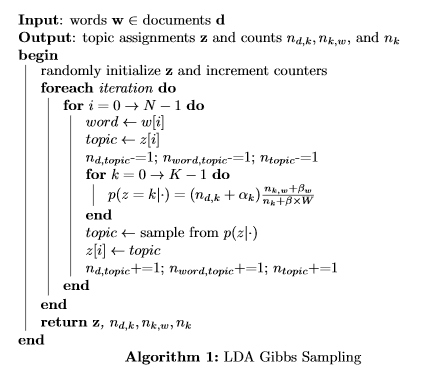
\includegraphics[scale=0.8]{./Slike/slika30.png} 
  \caption{Псеудокод - преузето са \cite{verov10} }\label{fig:slika27}
\end{figure}

